\documentclass[
	a4paper,
	parskip
]{scrartcl}

\usepackage[english]{babel}
\usepackage{authblk}
\usepackage{amsthm}
\usepackage{amsmath}
\usepackage{amssymb}
\usepackage{booktabs}
\usepackage{float}
\usepackage{multirow}
\usepackage{enumitem}
\usepackage{physics}
\usepackage{siunitx}
\usepackage{hyperref}
\usepackage{cleveref}
\usepackage{subcaption}
\usepackage{pgfplots}
\usepackage[
  backend=biber,
  sorting=none
]{biblatex}
\usepackage{csquotes}
\usepackage[american]{circuitikz}
\usepackage{glossaries}
\usepackage[subpreambles=true]{standalone}

\addbibresource{literature.bib}

\makeglossaries
\newglossaryentry{s5990}{name=S5990, description={Hamamatsu two-dimensional PSD}}
\newacronym{ic}{IC}{integrated circuit}
\newacronym{psd}{PSD}{position-sensitive detector}
\newacronym{gbp}{GBP}{gain-bandwidth-product}
\newacronym{pcb}{PCB}{printed circuit board}
\newacronym{bom}{BOM}{bill of materials}
\newacronym{smd}{SMD}{surface mounted device}
\newacronym{sma}{SMA}{SubMiniature version A}
\newacronym{html}{HTML}{hypertext markup language}

\pgfplotsset{compat=1.17}

\graphicspath{{image/}}

% https://tex.stackexchange.com/questions/247681/how-to-create-checkbox-todo-list/313337
\newlist{todolist}{itemize}{2}
\setlist[todolist]{label=$\square$}

\title{Position-sensitive device}
\author{Bodo Kaiser}
\affil{Ludwig-Maximilians-Universität München}
\affil{\textit{bodo.kaiser@physik.uni-muenchen.de}}

\begin{document}

\maketitle
\tableofcontents

\section{Introduction}

We define a position-sensitive device as a device that outputs voltages proportional to the center of mass coordinates of a light beam incident on a sensitive area.

The present document summarizes the insights acquired on the journey of building such a device.

\subsection{Motivation}

Position-sensitive devices are used in a wide range of industrial and commercial applications, including displacement sensing and beam alignment, see Ref.~\cite[p.~22]{Maekynen00}.

We are interested in using a position-sensitive device for beam pointing alignment in our quantum optics laboratory.

The beam pointing refers to a laser beam's spatial focus and can change through thermal and mechanical effects.
Uncompensated changes in beam alignment can quickly degrade the overall performance of an optical system.
Therefore, it is crucial to align the beam pointing to ensure the optical system's proper operation at hand.

\subsection{Overview}

This document is organized as follows.

The first two sections introduce the theory of the (position-sensitive) photodiode and the operational amplifier.
These sections are rather elaborate and should be skipped by the pragmatic scientist.

The third section describes the (electrical) schematics of the detector.
If you want to adjust parameters, e.g., gain or bandwidth, you should read these sections.

The fourth section is the only significant section if you want to build a \gls{psd}.
If you also want an example of using the \gls{psd} in an optical setup to determine the spatial resolution, you should also read the fifth section.
Finally, the appendix gives some guidance on troubleshooting.

\subsection{Requirements}

The requirements are specified rather loose. The only hard requirement concerns the connectors and voltages of the power supply. The power connector should be a LEMO4 whose pin configuration is compatible with the \SI{\pm15}{\volt} dual-voltage power supplies used in the labs. Features that would be nice to have are:
\begin{enumerate}
	\item The device should be sensible with optical powers that are safe to operate, i.e., $P<\SI{1}{\micro\watt}$. There is no preferred wavelength.
	\item For easy integration into existing optical setups, the device should be as compact as possible. Additional space, if needed, should be occupied by elonging the height. The sensitive area of the detector should be on the bottom. The connectors should be on the top to avoid cables blocking the beam path.
	\item It should be possible to mount different detector sizes on the device.
\end{enumerate}
The range of the output voltages of the device can be chosen for the optimal signal-to-noise ratio.

\subsection{Specification}

\begin{figure}[H]
	\centering
	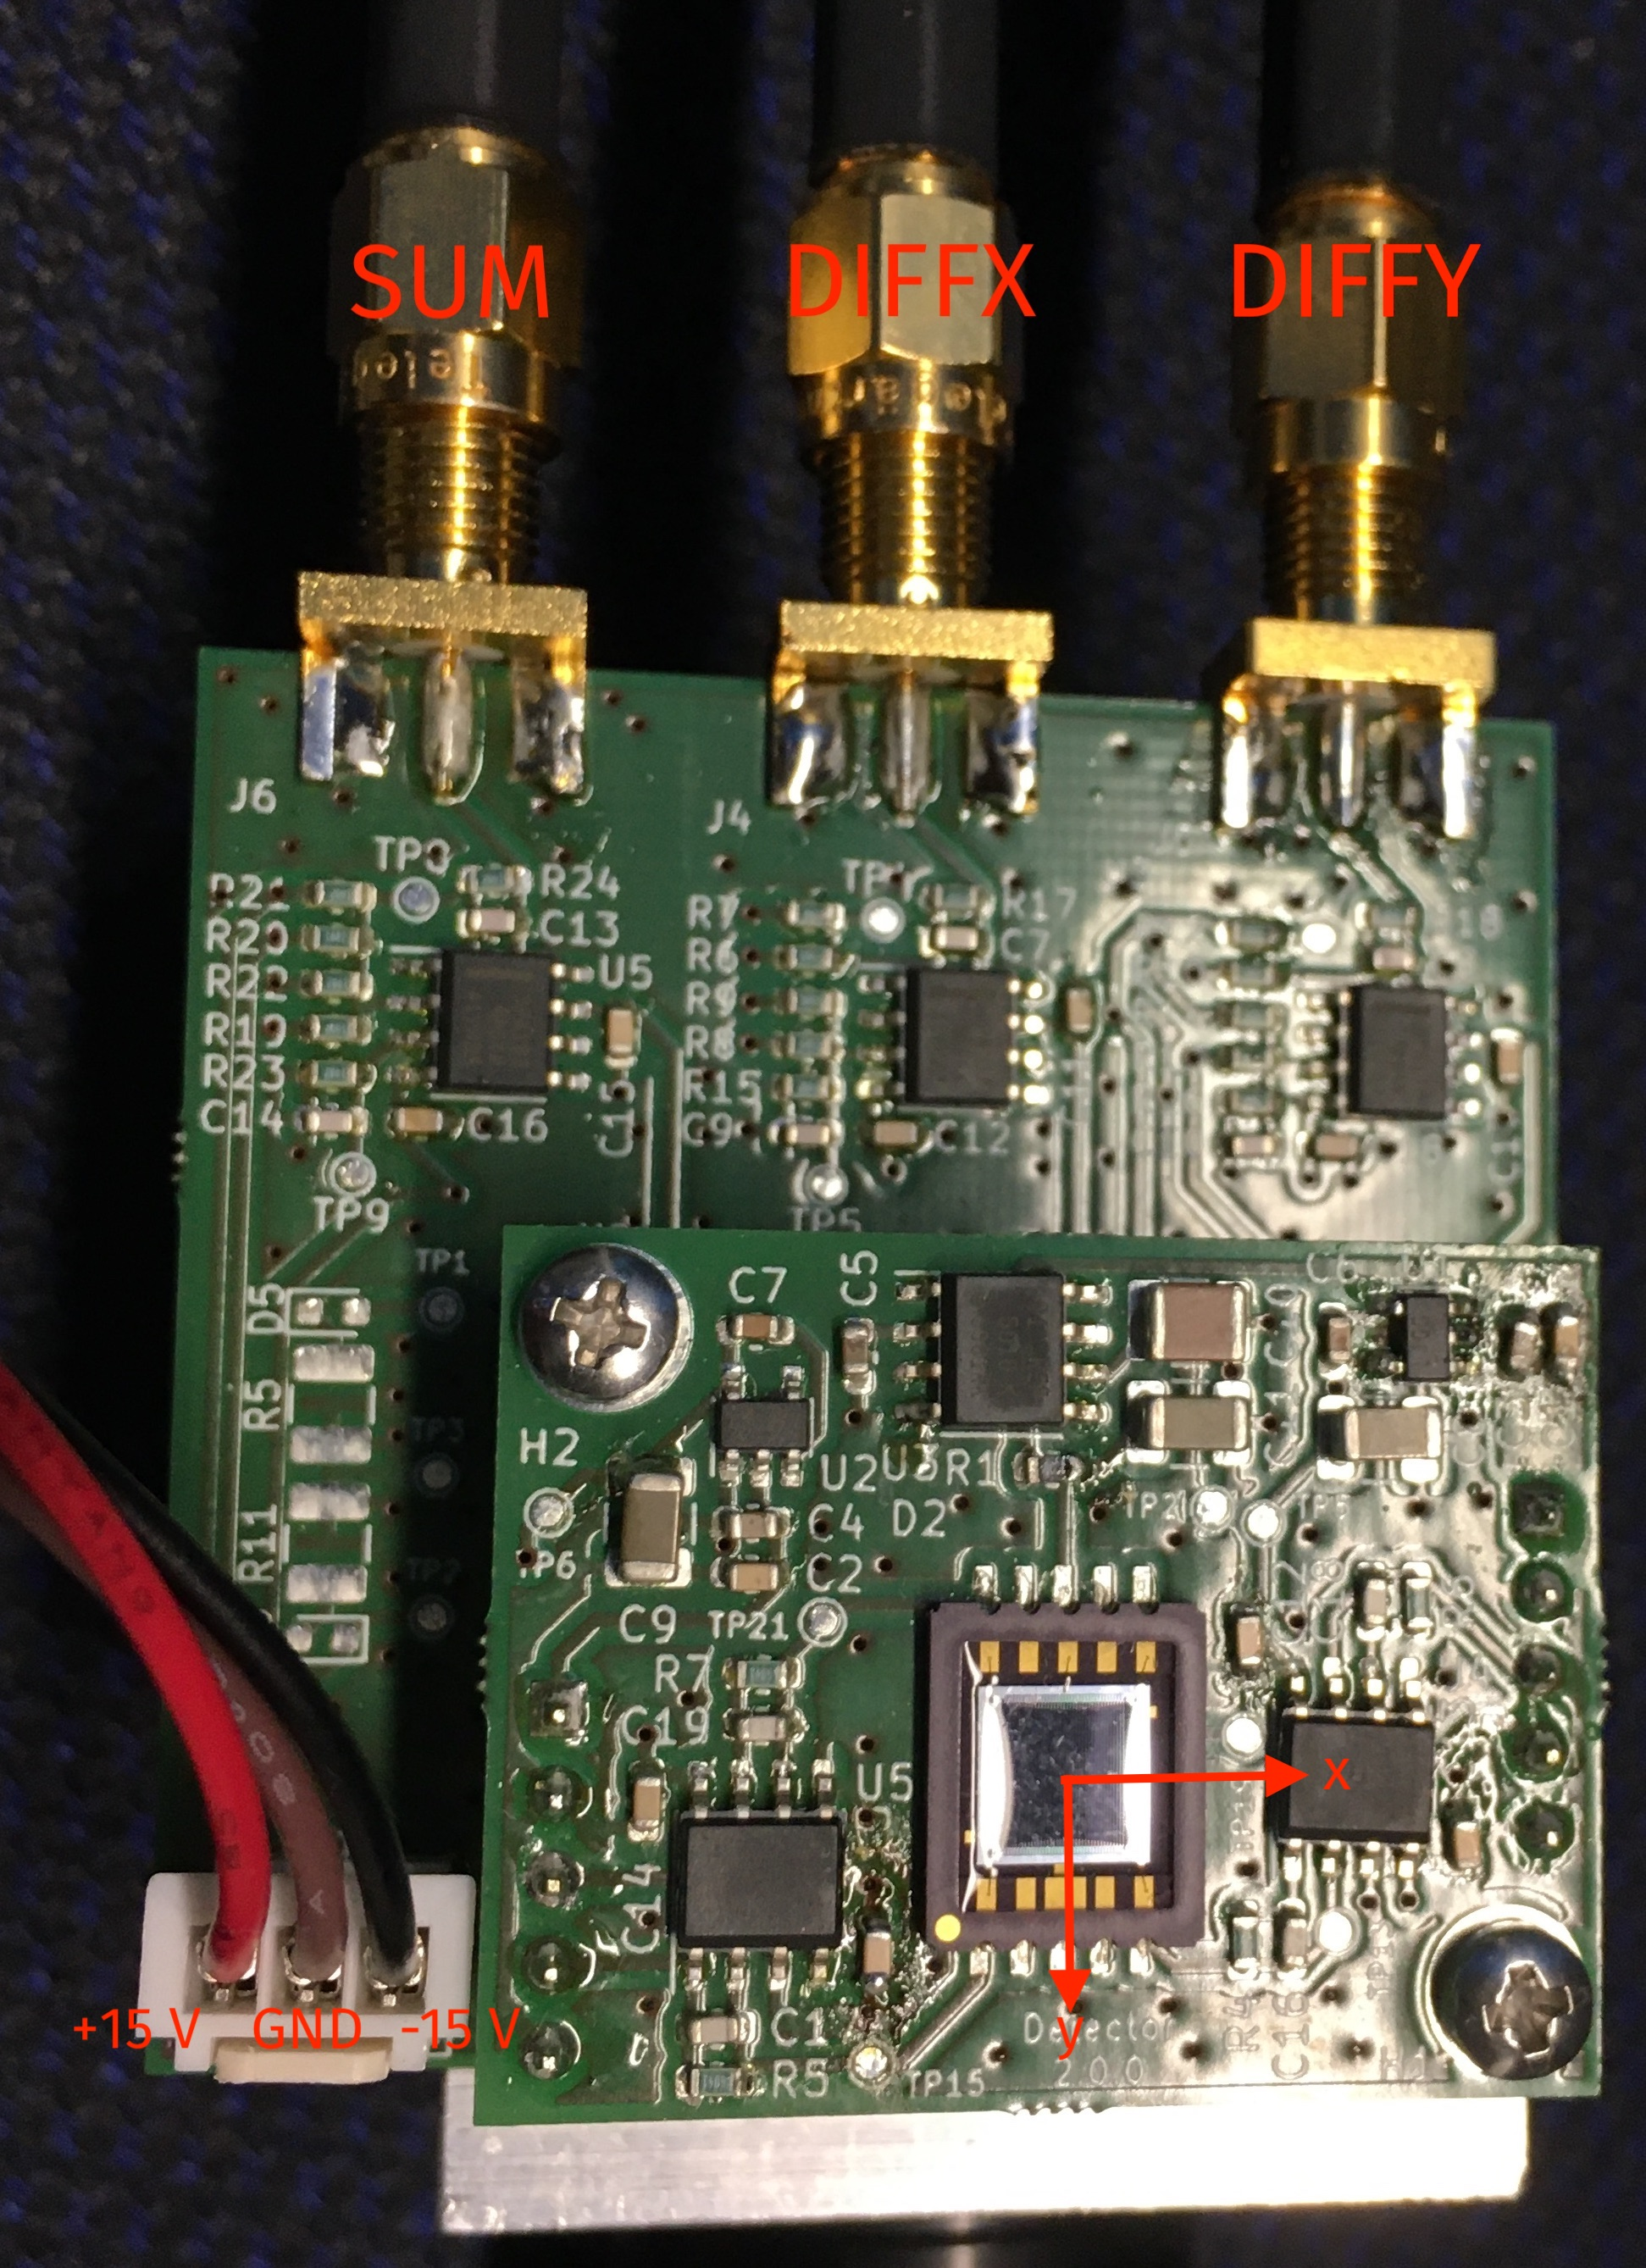
\includegraphics[scale=0.2]{detector.jpg}
	\caption{\gls{psd} on optical mount with connected cables}\label{fig:detector}
\end{figure}
\Cref{fig:detector} shows an image of the \gls{psd}.
The output voltage signals can be tapped from the upper \gls{sma} connectors.
The upper left connector gives the SUM voltage which reflects the total intensity of the optical signal.
The upper center connector gives the DIFFX voltage which reflects the difference proportional to the horizontal position on the sensitive area.
The upper right connector gives the DIFFY voltage which is proportional to the vertical position.
The SUM voltage is required to normalize the difference signals.
The DIFFX voltage increases when moving the light beam on the sensitive area to the right while the DIFFY voltage increases while moving the light beam to the bottom.
The device is powered by a 3-pin connector.
The outer (left) cable is the positive \SI{+15}{\volt} supply while the opposite cable is negative \SI{-15}{\volt} supply.
The center cable of the 3-pin connector has to reference ground.
The power connector has no polarity protection so be careful!

\begin{table}[htb]
  \centering
  \begin{tabular}{lcccc}
    \toprule
      Parameter & Minimum & Typical & Maximum \\
    \midrule
      Output voltages & \SI{-13}{\volt} & \SIrange{-2}{+2}{\volt} & \SI{+13}{\volt} \\
      Supply voltages & \SI{\pm13}{\volt} & \SI{\pm15}{\volt} & \SI{\pm37}{\volt} \\
      Spatial resolution & \SI{5.0}{\micro\meter} & \SI{2}{\micro\meter} & \SI{1}{\micro\meter} \\
      Bandwidth & & \SI{1400}{\kilo\hertz} & \\
    \bottomrule
  \end{tabular}
  \captionsetup{width=.8\textwidth}
  \caption{Specifications of the presented \gls{psd}}\label{tab:specifications}
\end{table}
\Cref{tab:specifications} summarizes the specifications of the presented \gls{psd}.
These specifications are only a rough estimate and we only assembled one \gls{psd} so far.
\section{Schematic}

The present section discusses some critical sections of the electrical schematics and should read for reference if parameters need to be adjusted.

\subsection{Photodiode frontend}

The design of the operational amplifier circuits is critical for the performance of the detector.
In the following section, we give a very brief summary of the design and the chosen parameters, which should be sufficient for someone familiar with operational amplifiers.

\begin{figure}[H]
	\centering
	\includestandalone[mode=buildnew]{figure/circuit/amplifier-transimpedance-input-capacitance}
 	\caption{Transimpedance amplifier for photodiode}\label{fig:transimpedance_amplifier}
\end{figure}

\subsection{Voltage regulator}

We use two voltage regulators to maintain a constant voltage of \SI{\pm12}{\volt} from the external \SI{\pm15}{\volt} power supply. The \SI{\pm12}{\volt} voltage powers most components except the transimpedance amplifiers of the detector.
Using a dedicated pair of voltage regulators to power the transimpedance amplifiers decreases the load on the primary voltage regulator.

\begin{figure}[H]
	\centering
	\includestandalone[mode=buildnew]{figure/circuit/voltage-regulator}
	\caption{Dual supply voltage regulator.}\label{fig:voltage_regulator_dual}
\end{figure}
\Cref{fig:voltage_regulator_dual} shows the circuitry of the primary voltage regulators that output \SI{\pm12}{\volt}.

\subsection{Voltage reference}

\subsection{Analog arithmetic}

\section{Production}

The manufacturing of the position-sensitive device involves the necessary steps to assemble the detector and arithmetic PCB.

It's best first to do the arithmetic board and if it works, proceed with the detector. Of course, if you only need one of the boards, perform the following steps only once.

\subsection{Commissioning}

Before we can assemble the PCBs, we need to gather the required components and order missing pieces.

The list of the required components is usually known as the bill of materials (BOM). You can generate a current BOM directly from the Kicad files by using the InteractiveHTML plugin. The plugin generates an HTML file that lists the components and their respective placement on the PCB. Furthermore, you can check if the parts are stocked and placed. Start by checking the local inventory for the components listed by the generated HTML BOM.

If certain elements are missing, you can check the BOM.xlsx file inside the project repository. It contains part numbers and product links from major electronic distributors. If you order, double-check the part of the BOM.xlsx with the generated HTML BOM, there might be errors, e.g., wrong casing sizes in the BOM.xlsx as the BOM.xslx is older.

Finally, it would be best to have the boxes for all the required components in front of you and marking them as sourced in the generated HTML BOM.

\subsection{Manufacturing}

After you sourced the components, you can place them using the solder paste on the PCB.

Put on rubber gloves as the solder paste is potentially hazardous. Take out the solder paste from the fridge and let it reach room temperature. It is possible to use the cold solder paste directly, but it makes the handling more difficult as the paste is less fluid.

Place the solder paste onto the contacts of the PCB. Generally speaking, it is better to have too much solder paste then too less. If there is a small overlap between the contacts, this is fine as the solder will shrink when transitioning to a liquid phase in the oven.

Now, place the SMD components onto the solder with a tweezer. For me, it works best to start with the larger components and then progress to the smaller ones. You can check the components as placed in the generated HTML BOM.

%\subsection{Reflow soldering}

Start the oven and adjust the frame on which you place the board with the screw to the appropriate size. Use an empty PCB for this.
After that, select the profile SMD180 and follow the instructions of the oven.

\subsection{Quality control}

Inspect the board for misplaced components and unmelted solder. You can use the solder heat gun to melt the remaining solder paste or remove misplaced components. However, you might blow away small capacitors.
You can fix other defects by hand soldering.

% \subsection{Hand soldering}

Some components, for example, the SMA mounts or the pin headers, have to be soldered by hand. Before soldering these components by hand, jump to the electrical testing section. Only, if your board passes the electrical tests, proceed with hand soldering the missing parts.

\subsection{Electrical testing}

With the electrical testing, we want to confirm that the solder connections and components work as expected.
The most basic check is that the supply voltages are correct.
More elaborated checks concern the operational amplifiers but are out of the scope of this document.

% \subsubsection{Arithmetic board I}

Leave the arithmetic board unpowered and measure the resistance between the supply lines through the test points TP1 (+12 V), TP2 (GND), and TP3 (-12 V).
There should be very high resistance between any of these test points.
Otherwise, there is a short.

If no short is detected, you can configure the power supply to provide a dual voltage of +- 15 V.
Alternatively, use two single voltage sources set to 15 V and connect the negative port of one of the voltage sources with the other one's positive voltage.
Confirm that the output voltages are correct with the multimeter. If possible, limit the current of the voltage sources.
You can set the current limit as low as possible and increase from there until the voltage becomes stable.
You might need to adjust the limit when connecting the voltages with the arithmetic board.

Connect the power supply with the arithmetic board but double-check the polarity.
The voltage between TP2 (GND) and TP1 (+12 V) should read around + 12 V while the voltage between TP2 (GND) and TP3 (- 12 V) should read about - 12 V.

Confirm that the supply voltages reach the op-amps.
Check the temperature of the op-amps.
If the op-amps are very hot, there is a short.
You can additionally check if the op-amps work by grounding the inverting input.
Because the op-amp's non-inverting input is connected with the ground, the op-amp output should be a virtual ground.

% \subsubsection{Detector board}

Have the detector board unplugged and measure the resistance between GND (you can use the center pin of the headers), TP5 (+ 5V), and TP6 (-5 V). If the resistance is high, proceed. Otherwise, find the short.

Measure the voltage between the photodiode and GND's outer pins while illuminating the sensitive area of the photodiode with a laser pointer.
You should detect a small voltage.

If the preceding checks are successful, mount the detector board on the arithmetic board, and measure the detector board's supply voltages.

Finally, confirm that the voltage reference (U3) outputs 10 V and that the op-amps have the correct supply voltage.

% \subsubsection{Arithmetic board II}

Leave the detector board mounted on the arithmetic board.
Measure the voltage at the outputs of the operational amplifiers of the arithmetic board.
For the summing amplifier (U5), we expect an increase in voltage when illuminating the photodiode with the laser pointer.
For the difference amplifiers (U3, U4), we expect the voltage to change when moving the laser pointer's focal spot on the photodiode.


\section{Usage}

\subsection{Setup}

% TODO: what equipment is needed
% TODO: how to wire the photodiode
% TODO: optical setup

\begin{figure}[H]
	\centering
	\includestandalone[mode=buildnew]{figure/optic/setup}
	\caption{Optical setup for testing}\label{fig:optical_setup}
\end{figure}

\subsection{Resolution}

% TODO: how to determine resolution of the detector

\appendix
\section{Theory of photodiode operation}

\subsection{Transverse photodiodes}

The purpose of the following section is to recall the mechanics of the (transverse) photoeffect observed in an illuminated p-n junction.
Figures and the description thereof is largely based on Ref.~\cite{Simon13}.
A subtle difference in the depicted figures and the figures of Ref.~\cite{Simon13} is that we exchanged the order of p- and n-type semiconductors.
We found this order to be more intuitive when referring to a p-n junction.

\Cref{fig:pn_junction_separated} shows a separated p- and n-type semiconductor.
In the upper half, we see an illustration of the p- and n-type semiconductor with their respective mobile charge carriers.
The p-type semiconductor has an excess of positive charge carriers (holes) which are depicted as white circles.
The n-type semiconductor has an excess of negative charge carriers (electrons) which are depicted as black circles.
The excess charge carriers form due to the implantation of acceptor and donator ions.
These are depicted as circles with plus and minus sign in \Cref{fig:pn_junction_separated}.
The implanted ions have more or fewer electrons than the atoms of the semiconductor material.
Therefore donating an electron or accepting an electron and effectively forming a hole as an absence of negative charge.
\begin{figure}[H]
	\centering
	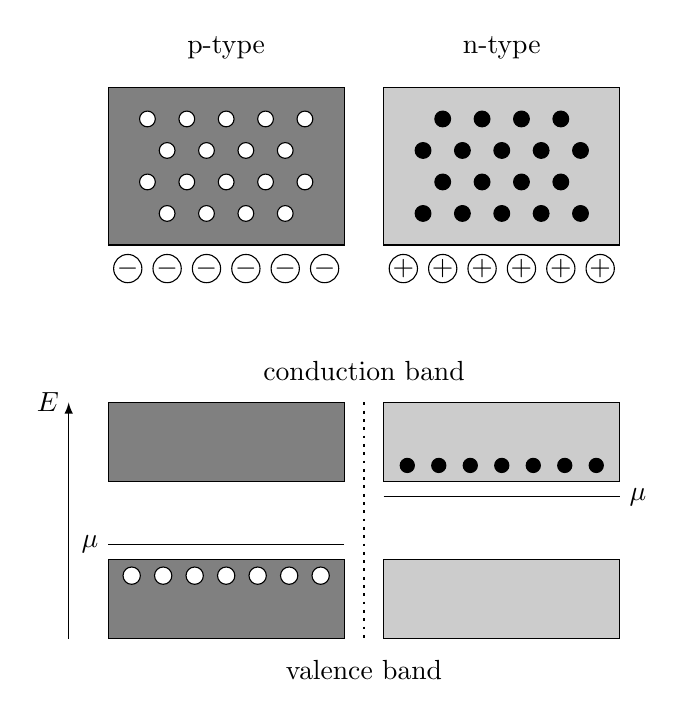
\begin{tikzpicture}
		\draw (1.5, 2.5) node {p-type};
		\draw (5, 2.5) node {n-type};
		\filldraw[draw=black, fill=gray] (0, 0) rectangle (3, 2);
		\filldraw[draw=black, fill=gray!40] (3.5, 0) rectangle (6.5, 2);
		\foreach \x in {1, ..., 4} {
			\filldraw[fill=white] (0.25+0.5*\x, 0.4) circle (.1);
			\filldraw[fill=white] (0.25+0.5*\x, 1.2) circle (.1);

			\filldraw[fill=black] (3.75+0.5*\x, 0.8) circle (.1);
			\filldraw[fill=black] (3.75+0.5*\x, 1.6) circle (.1);
		}
		\foreach \x in {1, ..., 5} {
			\filldraw[fill=white] (0.5*\x, 0.8) circle (.1);
			\filldraw[fill=white] (0.5*\x, 1.6) circle (.1);
			
			\filldraw[fill=black] (3.5+0.5*\x, 0.4) circle (.1);
			\filldraw[fill=black] (3.5+0.5*\x, 1.2) circle (.1);
		}
		\foreach \x in {0, ..., 5} {
			\draw (0.25+0.5*\x, -0.3) node[circle, draw=black, inner sep=0]{$-$};
			\draw (3.75+0.5*\x, -0.3) node[circle, draw=black, inner sep=0]{$+$};
		}
		\draw[-latex] (-0.5, -5) -- (-0.5, -2) node[left]{$E$};
		\draw[dotted, line width=1] (3.25, -2) -- (3.25, -5);
		\filldraw[draw=black, fill=gray] (0, -2) rectangle +(3, -1) +(0, -1.8) node[left]{$\mu$} -- +(3, -1.8) ++(0, -2) rectangle +(3, -1);
		\filldraw[draw=black, fill=gray!40] (3.5, -2) rectangle +(3, -1) +(0, -1.2) -- +(3, -1.2) node[right]{$\mu$} ++(0, -2) rectangle +(3, -1);
		\draw (3.25, -1.6) node{conduction band} +(0, -3.8) node{valence band};
		\foreach \x in {0, ..., 6} {
			\filldraw[fill=white] (0.3+0.4*\x, -4.2) circle (.11);
			\filldraw[fill=black] (3.8+0.4*\x, -2.8) circle (.09);
		}
	\end{tikzpicture}
	\caption{Separated p- and n-type semiconductor with holes (white) and electrons (black).}\label{fig:pn_junction_separated}
\end{figure}
The lower half of \Cref{fig:pn_junction_separated} shows the energy band structure of both p- and n-type semiconductor.
The lower energy band represents the valence band made up of the electrons that are tightly bound to a single atomic core.
The upper energy band represents the conduction band made up of electrons that are are not bound to a single atomic core but shared across the lattice.
Charge carriers in the conduction band can move freely and thereby contribute to the conductivity of the material.
For an undoped (intrinsic) semiconductor the chemical potential is in the center of the band gap between the conduction and valence band.
Through doping, the chemical potential is shifted in the p- and n-type semiconductor.
In the p-type semiconductor, acceptor ions can take up electrons from the conduction band, thereby decreasing the chemical potential.
In the n-type semiconductor, donator ions contribute electrons to the conduction band, thereby increasing the chemical potential.
\begin{figure}[H]
	\centering
	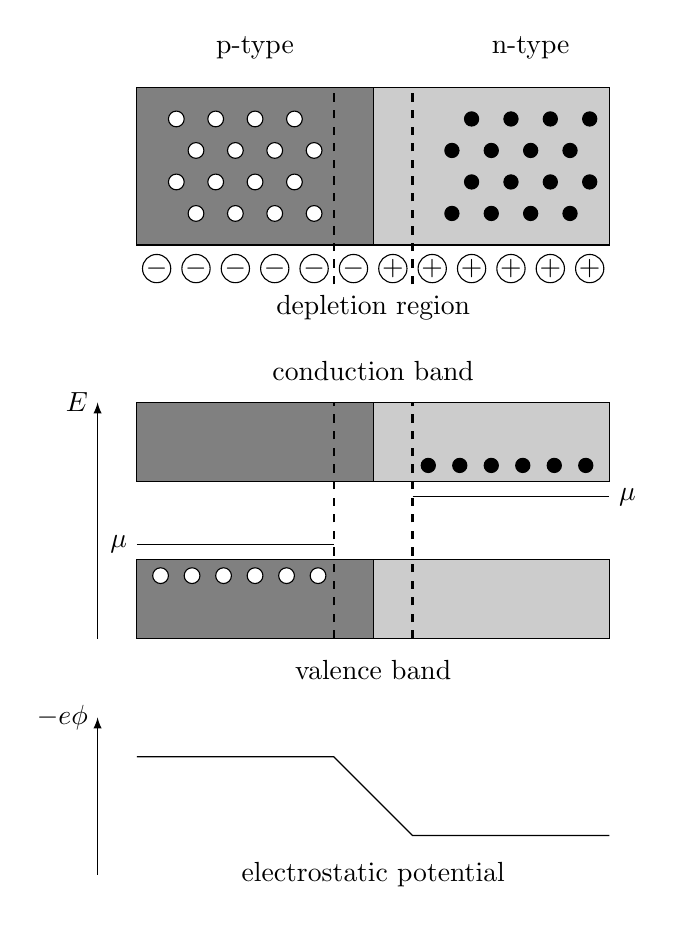
\begin{tikzpicture}
		\draw (1.5, 2.5) node {p-type};
		\draw (5, 2.5) node {n-type};
		\filldraw[draw=black, fill=gray] (0, 0) rectangle (3, 2);
		\filldraw[draw=black, fill=gray!40] (3, 0) rectangle (6, 2);
		\foreach \x in {1, ..., 4} {
			\filldraw[fill=white] (0.25+0.5*\x, 0.4) circle (.1);
			\filldraw[fill=white] (0.25+0.5*\x, 1.2) circle (.1);

			\filldraw[fill=black] (3.75+0.5*\x, 0.8) circle (.09);
			\filldraw[fill=black] (3.75+0.5*\x, 1.6) circle (.09);
		}
		\foreach \x in {1, ..., 4} {
			\filldraw[fill=white] (0.5*\x, 0.8) circle (.1);
			\filldraw[fill=white] (0.5*\x, 1.6) circle (.1);
			
			\filldraw[fill=black] (3.5+0.5*\x, 0.4) circle (.09);
			\filldraw[fill=black] (3.5+0.5*\x, 1.2) circle (.09);
		}
		\foreach \x in {0, ..., 5} {
			\draw (0.25+0.5*\x, -0.3) node[circle, draw=black, inner sep=0]{$-$};
			\draw (3.25+0.5*\x, -0.3) node[circle, draw=black, inner sep=0]{$+$};
		}
		\draw[dashed, line width=.8] (2.5, -.5) -- +(0, 2.5) +(1, 0) -- +(1, 2.5) +(0.5, -0.3) node{depletion region};

		\draw[-latex] (-0.5, -5) -- (-0.5, -2) node[left]{$E$};
		\filldraw[draw=black, fill=gray] (0, -2) rectangle +(3, -1) +(0, -1.8) node[left]{$\mu$} -- +(2.5, -1.8) ++(0, -2) rectangle +(3, -1);
		\filldraw[draw=black, fill=gray!40] (3, -2) rectangle +(3, -1) +(0.5, -1.2) -- +(3, -1.2) node[right]{$\mu$} ++(0, -2) rectangle +(3, -1);
		\draw[dashed, line width=.8] (2.5, -5) -- +(0, 3) +(1, 0) -- +(1, 3) +(0.5, -0.3);
		\draw (3, -1.6) node{conduction band} +(0, -3.8) node{valence band};
		\foreach \x in {0, ..., 5} {
			\filldraw[fill=white] (0.3+0.4*\x, -4.2) circle (.10);
			\filldraw[fill=black] (3.7+0.4*\x, -2.8) circle (.09);
		}
		
		\draw[-latex] (-0.5, -8) -- (-0.5, -6) node[left]{$-e\phi$};
		\draw (0, -6.5) -- ++(2.5, 0) -- ++(1, -1) -- ++(2.5, 0);
		\draw (3, -8) node{electrostatic potential};
	\end{tikzpicture}
	\caption{Combined p- and n-type semiconductor with holes (white) and electrons (black).}\label{fig:pn_junction_combined}
\end{figure}
In \Cref{fig:pn_junction_combined} the p- and n-type semiconductor are brought into contact with each other, forming a p-n junction.
In close proximity of the junction holes and energies recombine due to a diffusion process, leaving an electrically charged area.
The electrically charged area creates an electrostatic potential across the junction as illustrated in the lower part of \Cref{fig:pn_junction_combined}.
We refer to this area as the depletion region.
In \Cref{fig:pn_junction_combined} the depletion region expands between the dashed lines around the junction.
\begin{figure}[H]
	\centering
	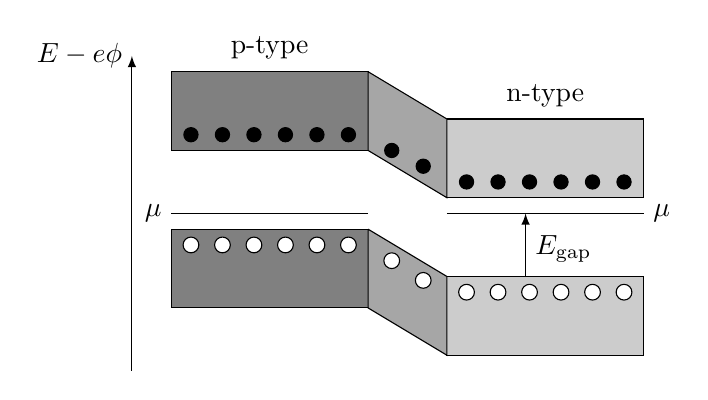
\begin{tikzpicture}
		\draw (1.25, 3.6) node {p-type};
		\draw (4.75, 3.0) node {n-type};
		\draw[-latex] (-0.5, -0.5) -- (-0.5, 3.5) node[left]{$E-e\phi$};
		\filldraw[draw=black, fill=gray] (0, 3.3) rectangle +(2.5, -1) +(0, -1.8) node[left]{$\mu$} -- +(2.5, -1.8) ++(0, -2) rectangle +(2.5, -1);
		\filldraw[draw=black, fill=gray!40] (3.5, 2.7) rectangle +(2.5, -1) +(0, -1.2) -- +(2.5, -1.2) node[right]{$\mu$} ++(0, -2) rectangle +(2.5, -1);
		\filldraw[draw=black, fill=gray!70] (2.5, 3.3) -- ++(1, -.6) -- ++(0, -1) -- ++(-1, .6) -- ++(0, 1);
		\filldraw[draw=black, fill=gray!70] (2.5, 1.3) -- ++(1, -.6) -- ++(0, -1) -- ++(-1, .6) -- ++(0, 1);
		\draw[-latex] (4.5, 0.7) -- ++(0, 0.8);
		\draw (4.5, 1.05) node[right]{$E_\text{gap}$};
		\foreach \x in {0, ..., 5} {
			\filldraw[fill=white] (0.25+0.4*\x, 1.1) circle (.10);
			\filldraw[fill=white] (3.75+0.4*\x, 0.5) circle (.10);
			\filldraw[fill=black] (3.75+0.4*\x, 1.9) circle (.09);
			\filldraw[fill=black] (0.25+0.4*\x, 2.5) circle (.09);
		};
		\filldraw[fill=white] (2.8, 0.9) circle (.10);
		\filldraw[fill=white] (3.2, 0.65) circle (.10);
		\filldraw[fill=black] (2.8, 2.3) circle (.09);
		\filldraw[fill=black] (3.2, 2.1) circle (.09);
	\end{tikzpicture}
	\caption{Energy bands of the p-n junction.}\label{fig:pn_junction}
\end{figure}
The energy band diagram in \Cref{fig:pn_junction} accounts for the shift in energy due to the electrostatic potential.
The chemical potentials of both sides of the junction are now aligned.
The energy required to excite an electron on the p-type side from the valence to the conduction band and the energy required to excite a hole from the conduction to the valence band are equal to the band gap of the semiconductor.

% TODO: motivate reverse bias (photoconductive mode) vs. unbiased (photovoltaic) mode by measurement vs. energy conversion application 
If one applies a reverse bias voltage across the p-n junction, the effective energy gap between conduction and valence band is reduced, the electrostatic potential increases and the depletion region broadens.
The situation of an applied reverse voltage is depicted in \Cref{fig:pn_junction_reverse}.
\begin{figure}[H]
	\centering
	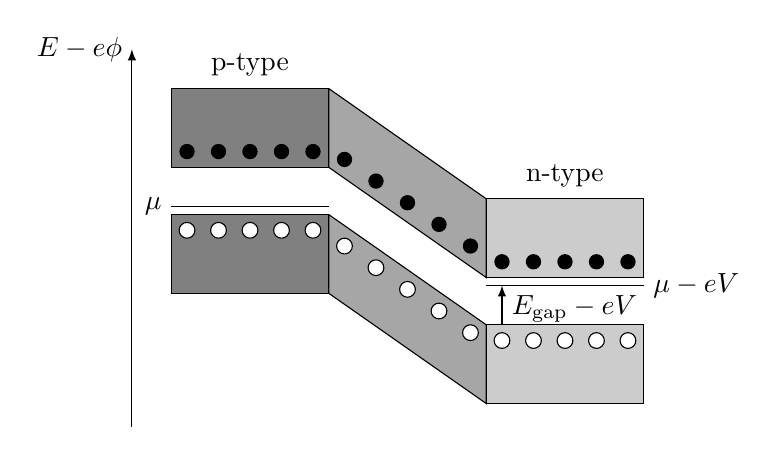
\begin{tikzpicture}
		\draw (1, 3.6) node {p-type};
		\draw (5, 2.2) node {n-type};
		\draw[-latex] (-0.5, -1) -- (-0.5, 3.8) node[left]{$E-e\phi$};
		\filldraw[draw=black, fill=gray] (0, 3.3) rectangle +(2, -1) +(0, -1.5) node[left]{$\mu$} -- +(2, -1.5) ++(0, -1.6) rectangle +(2, -1);
		\filldraw[draw=black, fill=gray!40] (4, 1.9) rectangle +(2, -1) +(0, -1.1) -- +(2, -1.1) node[right]{$\mu-eV$} ++(0, -1.6) rectangle +(2, -1);
		\filldraw[draw=black, fill=gray!70] (2, 3.3) -- ++(2, -1.4) -- ++(0, -1) -- ++(-2, 1.4) -- ++(0, 1);
		\filldraw[draw=black, fill=gray!70] (2, 1.7) -- ++(2, -1.4) -- ++(0, -1) -- ++(-2, 1.4) -- ++(0, 1);
		\draw[-latex] (4.2, 0.3) -- ++(0, 0.5);
		\draw (4.2, 0.5) node[right]{$E_\text{gap}-eV$};
		\foreach \x in {0, ..., 4} {
			\filldraw[fill=white] (0.2+0.4*\x, 1.5) circle (.10);
			\filldraw[fill=white] (2.2+0.4*\x, 1.3-0.275*\x) circle (.10);
			\filldraw[fill=white] (4.2+0.4*\x, 0.1) circle (.10);
			\filldraw[fill=black] (4.2+0.4*\x, 1.1) circle (.09);
			\filldraw[fill=black] (2.2+0.4*\x, 2.4-0.275*\x) circle (.09);
			\filldraw[fill=black] (0.2+0.4*\x, 2.5) circle (.09);
		};
	\end{tikzpicture}
	\caption{Energy band diagram of a reverse biased p-n junction.}\label{fig:pn_junction_reverse}
\end{figure}
The current-voltage characteristic of the p-n junction is described by the Schockley diode equation,
\begin{equation}
	I_\text{diode}=I_\text{sat}(T)\left(e^{eV/k_BT}-1\right)
	\label{eq:diode_current},
\end{equation}
wherein $I_\text{sat}\propto e^{-E_\text{gap}/k_BT}$ is the temperature dependent reverse bias saturation current and $V$ the voltage applied to the p-n junction.
Using the proportionality of the reverse bias saturation current, we can write,
\begin{equation}
	I_\text{diode}\propto e^{\left(eV-E_\text{gap}\right)/k_BT}-e^{-E_\text{gap}/k_BT}\label{eq:diode_current_prop},
\end{equation} 
which discloses the two effects contributing to the diode current.
The left-hand side of the proportionality of \Cref{eq:diode_current_prop} represents the current contribution due intra-band excitation of charge carriers, whereas the right-hand side represents the current contribution due to inter-band excitation.
\begin{figure}[H]
	\centering
	\begin{tikzpicture}
		\begin{axis}[xmin=-5, xmax=5, xticklabels=\empty, xlabel=$V$, ymin=-5, ymax=5, ylabel=$I$, yticklabels=\empty, axis lines=middle]
			\addplot[domain=-5:2, samples=100]{exp(x)-1-1/(x+5.4)^6};
			\addplot[domain=-5:2, samples=100]{exp(x)-1-1/(x+5.4)^6-0.5};
			\addplot[domain=-5:2, samples=100]{exp(x)-1-1/(x+5.4)^6-1};
		\end{axis}
		\draw (-0.2, 2.3) node[left]{$I_\text{sat}$} -- +(1.4, 0);
		\draw (-0.2, 1.72) node[left]{$I_\text{sat}-I_\text{photo}$} -- +(1.3, 0);
	\end{tikzpicture}
	\caption{Current-voltage characteristics of a p-n junction with different levels of illumination.}\label{fig:pn_junction_iv}
\end{figure}
In \Cref{fig:pn_junction_iv} we see the current-voltage characteristics of the p-n junction under different levels of illumination.
For negative voltages, the p-n junction is operated under reverse bias.
If the reverse bias voltage exceeds the breakdown voltage the p-n junction starts to conduct.
The current before the breakdown occurs is the reverse saturation current.
For different levels of illumination, the curve is shifted downwards.
The separation between the non-illuminated (top curve) and illuminated curves represent the respective photocurrent.

The conversion rate of photons to photoelectrons depends on the type of the band gap, i.e. direct or indirect, the wavelength $\lambda$ of the photon and the temperature $T$.
Most photodiodes report a wavelength $\lambda$ dependent responsitivity $R$ which can be used to convert the radiant flux $P$ of the incident light to the generated photocurrent $I_\text{photo}$,
\begin{equation}
	I_\text{photo}=R(\lambda)P
	\label{eq:responsitivity}.
\end{equation}
For silicon-based p-n junctions, the responsitivity $R(\lambda)$ is between \SI{0.2}{\ampere\per\watt} at \SI{400}{\nano\meter} and \SI{0.6}{\ampere\per\watt} at \SI{950}{\nano\meter}.

\begin{figure}[H]
	\centering
	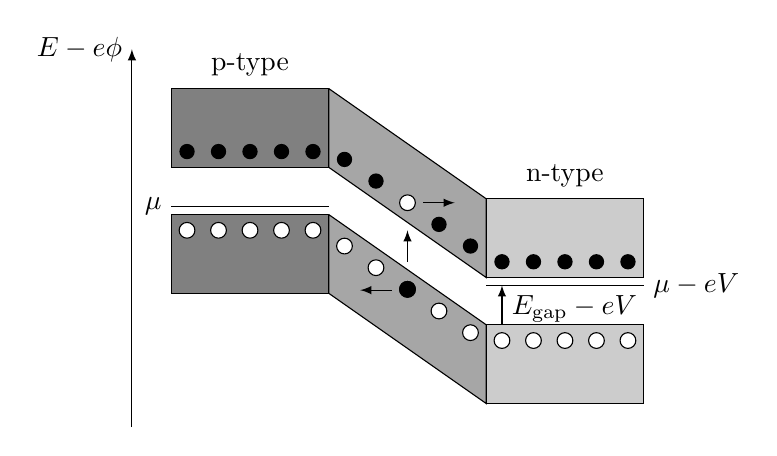
\begin{tikzpicture}
		\draw (1, 3.6) node {p-type};
		\draw (5, 2.2) node {n-type};
		\draw[-latex] (-0.5, -1) -- (-0.5, 3.8) node[left]{$E-e\phi$};
		\filldraw[draw=black, fill=gray] (0, 3.3) rectangle +(2, -1) +(0, -1.5) node[left]{$\mu$} -- +(2, -1.5) ++(0, -1.6) rectangle +(2, -1);
		\filldraw[draw=black, fill=gray!40] (4, 1.9) rectangle +(2, -1) +(0, -1.1) -- +(2, -1.1) node[right]{$\mu-eV$} ++(0, -1.6) rectangle +(2, -1);
		\filldraw[draw=black, fill=gray!70] (2, 3.3) -- ++(2, -1.4) -- ++(0, -1) -- ++(-2, 1.4) -- ++(0, 1);
		\filldraw[draw=black, fill=gray!70] (2, 1.7) -- ++(2, -1.4) -- ++(0, -1) -- ++(-2, 1.4) -- ++(0, 1);
		\draw[-latex] (4.2, 0.3) -- ++(0, 0.5);
		\draw (4.2, 0.5) node[right]{$E_\text{gap}-eV$};
		\foreach \x in {0, ..., 4} {
			\filldraw[fill=white] (0.2+0.4*\x, 1.5) circle (.10);
			\filldraw[fill=white] (2.2+0.4*\x, 1.3-0.275*\x) circle (.10);
			\filldraw[fill=white] (4.2+0.4*\x, 0.1) circle (.10);
			\filldraw[fill=black] (4.2+0.4*\x, 1.1) circle (.09);
			\filldraw[fill=black] (2.2+0.4*\x, 2.4-0.275*\x) circle (.09);
			\filldraw[fill=black] (0.2+0.4*\x, 2.5) circle (.09);
		};
		\filldraw[fill=white] (3.0, 1.85) circle (.10);
		\filldraw[fill=black] (3.0, 0.75) circle (.10);
		\draw[-latex] (3.0, 1.1) -- +(0, 0.4);
		\draw[-latex] (3.2, 1.85) -- +(0.4, 0);
		\draw[-latex] (2.8, 0.74) -- +(-0.4, 0);
	\end{tikzpicture}
	\caption{Energy diagram of a reverse biased p-n junction under illumination.}\label{fig:pn_junction_illumination}
\end{figure}
\Cref{fig:pn_junction_illumination} shows a p-n junction under reverse bias where a photon excites an electron-hole pair in the depletion region.
Due to the electrostatic potential, the electron is accelerated to the right side.
Analogue the hole is accelerated to the left side and in addition to the diode current, \Cref{eq:diode_current}, a photocurrent can be measured across the junction.

\subsection{Lateral photodiodes}

In the previous section, we discussed the transversal photoeffect that is usually associated with the illumination of the p-n junction.
In addition to the transversal photoeffect, the lateral photoeffect was first discovered by W. Schottky~\cite{Schottky30} in 1930 and later rediscovered in 1957 by J. Wallmark~\cite{Wallmark57}.
In the present section, we summarize important results from Ref.~\cite{Noorlag74} and Ref.~\cite{Woltring75} with focus on the tetralateral photodiode which is the most common commercially available design.
\begin{figure}[H]
	\centering
	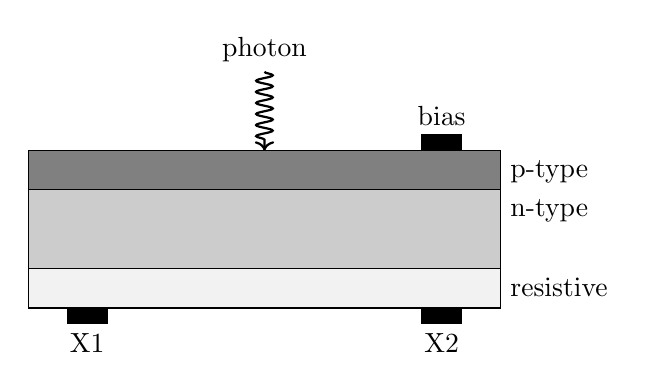
\begin{tikzpicture}
		\filldraw[fill=gray] (0, 1.5) rectangle +(6, 0.5) node[below right]{p-type};
		\filldraw[fill=gray!40] (0, 0.5) rectangle +(6, 1) node[below right]{n-type};
		\filldraw[fill=gray!10] (0, 0) rectangle +(6, 0.5) node[below right]{resistive};
		\filldraw[fill=black] (5, 2) rectangle ++(0.5, 0.2) +(-0.25, 0) node[above]{bias};
		\draw [->, thick, decorate, decoration={snake, amplitude=3, segment length=4, post length=3}] (3, 3) node[above]{photon} -- +(0, -1);
		\filldraw[fill=black] (0.5, 0) rectangle ++(0.5, -0.2) +(-0.25, 0) node[below]{X1};
		\filldraw[fill=black] (5, 0) rectangle ++(0.5, -0.2) +(-0.25, 0) node[below]{X2};
	\end{tikzpicture}
	\caption{Cross section of a lateral photodiode.}\label{fig:lateral_photodiode_cross_section}
\end{figure}
\Cref{fig:lateral_photodiode_cross_section} depicts the cross-section of a lateral photodiode with a p-type semiconductor as the top, an n-type semiconductor as the middle layer and a resistive material as the bottom layer.
An electric contact embedded into the top layer can be used as a common cathode.
The common cathode can be connected to the ground or a positive voltage for reverse bias operation.
In contrast to the transversal photodiode, the lateral photodiode has two anode contacts positioned at the opposite sites embedded into the resistive layer.
The photocurrent measured at each of the anode contacts follows an almost linear relationship with the center-of-mass of the incident light spot.
Therefore the lateral photodiode can be used to measure the spatial coordinate of an incident light spot.

The dynamics of the lateral photodiode are guided by the Lucovsky~\cite{Lucovsky60} equation,
\begin{equation}
	\nabla^2V=\frac{\rho}{w}J_s\left(e^{eV/k_BT}-1\right)-\frac{\rho_d}{w}J_p\label{eq:lucovsky_exact},
\end{equation}
wherein $V$ is the diode voltage, $\rho$ is the resistance per unit length of the resistive layer, $J_s$ is the reverse-bias saturation current and $J_p$ is the photocurrent generated due photon induced electron-hole excitation.
\Cref{eq:lucovsky_exact} can be obtained by combination of the current density continuity equation with Ohm's law and the Schottky equation, \Cref{eq:diode_current}.

According to Ref.~\cite{Woltring75}, operation of the lateral in fully reverse-bias has the following benefits:
\begin{enumerate}
	\item Reduced signal loss.
	\item Improved response speed and resolution.
	\item Improved linearity of the position.
	\item Reduced temperature dependence.
\end{enumerate}
In electronic engineering literature, e.g. Ref.~\cite[p.~258]{Jung05}, one is sometimes discouraged from operating a photodiode under reverse-bias for highest sensitivity as the reverse-bias increased the diode leakage (dark) current.
We believe that as long as the dark current is significantly smaller than the typical photocurrent, the photodiode should always be operated in reverse-bias mode as recommended Ref.~\cite{Noorlag74,Woltring75,Wang89,Hobbs11}.

Assuming a fully reverse-biased lateral photodiode, we have $eV/k_BT\ll1$ and \Cref{eq:lucovsky_exact} simplifies to a linear second order differential (Poisson) equation,
\begin{equation}
	\nabla^2V\approx-\frac{\rho}{w}\left(J_s+J_p\right)
	\label{eq:lucovsky_reverse_bias},
\end{equation}
which can be solved using variable separation and a product Ansatz.
The solution of \Cref{eq:lucovsky_reverse_bias} depends on the imposed boundary conditions.
The Dirichlet boundary condition, $V=0$, should be used if an electrical contact terminates the semiconductor, otherwise, the Neumann boundary condition, $\pdv{V}{n}=0$, should be assumed.
\begin{figure}[H]
	\centering
	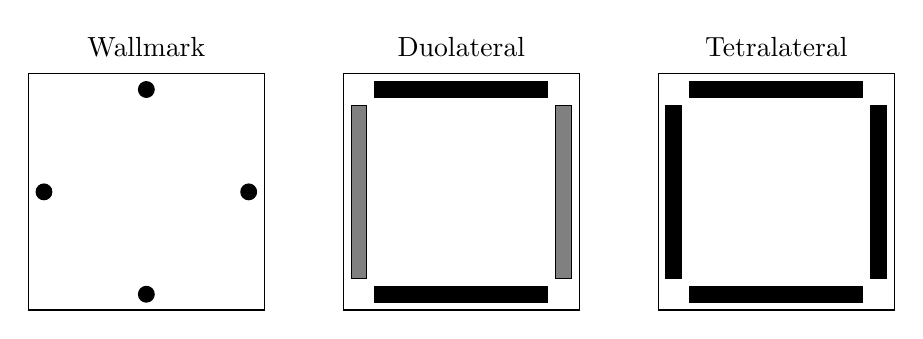
\begin{tikzpicture}
		\filldraw[fill=white] (0, 0) rectangle +(3, 3);
		\filldraw[fill=white] (4, 0) rectangle +(3, 3);
		\filldraw[fill=white] (8, 0) rectangle +(3, 3);
		\filldraw (1.5, 0.2) circle (.1);
		\filldraw (1.5, 2.8) circle (.1);
		\filldraw (0.2, 1.5) circle (.1);
		\filldraw (2.8, 1.5) circle (.1);
		\filldraw (4.4, 0.1) rectangle (6.6, 0.3);
		\filldraw (4.4, 2.7) rectangle (6.6, 2.9);
		\filldraw[fill=black!50] (4.1, 0.4) rectangle (4.3, 2.6);
		\filldraw[fill=black!50] (6.7, 0.4) rectangle (6.9, 2.6);
		\filldraw (8.4, 0.1) rectangle (10.6, 0.3);
		\filldraw (8.4, 2.7) rectangle (10.6, 2.9);
		\filldraw (8.1, 0.4) rectangle (8.3, 2.6);
		\filldraw (10.7, 0.4) rectangle (10.9, 2.6);
		\draw (1.5, 3.1) node[above]{Wallmark};
		\draw (5.5, 3.1) node[above]{Duolateral};
		\draw (9.5, 3.1) node[above]{Tetralateral};
	\end{tikzpicture}
	\caption{Contact configurations of a lateral photodiode.}\label{fig:lateral_photodiode_contacts}
\end{figure}
In \Cref{fig:lateral_photodiode_contacts} we present three different contact configurations.
The left contact configuration was used by Wallmark~\cite{Wallmark57} and comprises four small electronic contacts.
Assuming that the contact size is small compared to the surface of the photodiode, the von Neumann boundary condition have to be used.
The middle contact configuration receives great attention from Noorlag~\cite{Noorlag74}.
On two opposite sides of the photodiode an electric contact terminates the boundary while the remaining sides are left empty.
For two-dimensional position detection, one can create two electric contacts at another layer.
Mathematically we can express this configuration as combination of Neumann and Dirichlet boundary conditions.
Finally, the tetralateral configuration where each side on the same layer is terminated by electric contacts can be modelled by Dirichlet boundary conditions on all sides.
For a rectangular tetralateral photodiode of width $l$, the explicit boundary conditions are,
\begin{align}
	V(0, y)=V(l,y)=0, && V(x,0)=V(x,l)=0.
\end{align}
Together with the initial condition that a focused light spot hits the photodiode at $(x^*,y^*)$,
\begin{equation}
	V_p(x,y, t=0)=I_p\frac{\rho}{w}\delta(x-x^*)\delta(y-y^*)
	\label{eq:lucovsky_initial},
\end{equation}
the general solution of the Lucovsky equation, \Cref{eq:lucovsky_reverse_bias}, for the tetralateral configuration reads,
\begin{equation}
	V^*_p(x,y)=I_p\frac{\rho}{w}\sum_{n\in\mathbb{Z}}\sum_{m\in\mathbb{Z}}\frac{\sin(m\pi x/l)\sin(m\pi x^*/l)\sin(n\pi y/l)\sin(n\pi y^*/l)}{(m^2+n^2)\pi^2}
	\label{eq:lucovsky_solution}.
\end{equation}
The current that flows through the $x1$ contact is given by,
\begin{equation}
	I_{x1}(x^*,y^*)=\frac{w}{\rho}\int_0^l\dd{y}\eval{\pdv{V}{x}}_{x=0},
\end{equation}
respective,
\begin{equation}
	I_{x1}(x^*,y^*)=\frac{2}{\pi}I_p\sum_{n\in\mathbb{Z}}\frac{\sin[(2n-1)\pi y^*/l]}{2n-1}\frac{\sinh[\abs{2n-1}\pi(1-x^*/l)]}{\sinh(\abs{2n-1}\pi)}
	\label{eq:lucovsky_current}.
\end{equation}
The solution does not disclose the linear relationship between anode current $I_{x1}$ and the incident spot light coordinate $x^*$.
Ref.~\cite[Fig.~7]{Woltring75} renders the non-linear distortion close to the boundaries as described by \Cref{eq:lucovsky_current}.
In order to show analytically that there is an almost linear relationship between $I_{x1}$ and $x^*$, we fix $y^*=l/2$, numerically evaluate the dominant terms and Taylor expand the terms to linear order,
\begin{align}
	I_{x1}(x^*,l/2)
	&=\frac{2}{\pi}I_p\sum_{n\in\mathbb{Z}}\frac{(-1)^{n+1}}{2n-1}\frac{\sinh(\abs{2n-1}\pi(1-x^*/l))}{\sinh(\abs{2n-1}\pi)}\\
	&\approx I_p\left\{0.25-0.41731\left(\frac{x}{2l}-1\right)\right\}+\mathcal{O}\left(\left(\frac{x^*}{l}-\frac{1}{2}\right)^2\right).
\end{align}
Using the difference between two opposite contacts and normalizing for the total photocurrent, we find,
\begin{equation}
	\frac{I_{x2}(x^*,l/2)-I_{x1}(x^*,l/2)}{I_{x1}(x^*,l/2)+I_{x2}(x^*,l/2)}
	\propto\frac{x}{l},
\end{equation}
which indeed is linear in $x$.

According to Ref.~\cite[p.~41]{Noorlag74}, the tetralateral photodiode has benefits in manufacturing, although its linearity is below the duallateral photodiode, but still better than the Wallmark type, see Ref.~\cite{Woltring75}.
Recent contact configurations have improved upon the tetralateral design in order to improve the linearity.
For example, the commercially availble pin-cushion tetralateral photodiode, discussed in Ref.~\cite{Doke87,Wang89}, shows good linearity over a large area.
The center-of-mass of an incident light spot at $(x^*,y^*)$ can be recovered from the anode currents via,
\begin{align}
	\frac{\left(I_{x2}+I_{y1}\right)-\left(I_{x1}+I_{y2}\right)}{I_{x1}+I_{x2}+I_{y1}+I_{y2}}=\frac{2x^*}{l} &&
	\frac{\left(I_{x2}+I_{y2}\right)-\left(I_{x1}+I_{y1}\right)}{I_{x1}+I_{x2}+I_{y1}+I_{y2}}=\frac{2y^*}{l}	.
\end{align}
The datasheet~\cite{HamamatsuS5990} of the \gls{s5990}, a pin-cushion tetralateral photodiode, discloses the position detectability of a light spot of size \SI{0.2}{\milli\meter} over a scan interval of \SI{0.4}{\milli\meter} which does not show any non-linear distortion.

\subsection{Equivalent circuit}

In the previous section, we described the physics behind the lateral photodiode.
In the current section, we want to ignore microscopic details and concentrate on the electrical properties of real tetralateral photodiodes.

In \Cref{fig:tetralateral_photodiode_equivalent} the equivalent circuit of a tetralateral photodiode is depicted.
The tetralateral photodiode has four anode connections X1, X2, Y1, and Y2 which are connected to the junction via position-dependent resistances $R_1$, $R_2$, $R_3$, and $R_4$.
The actual junction is equivalent to two current sources $I_p,I_d$, a resistor $R_d$, and a capacitor $C_d$ in parallel.
The first current source $I_p$ represents the generated photocurrent with typical values between \si{\micro\ampere} and \si{\milli\ampere}.
The second current source $I_d$ represents the generated leakage or dark current with typical values between \si{\pico\ampere} and \si{\nano\ampere}.
\begin{figure}[H]
	\centering
	\begin{circuitikz}
		\draw (-3, -2) to[current source, l=$I_p$] ++(0, 4);
		\draw (-1, -2) node[circ]{} to[current source, l=$I_d$] ++(0, 4) node[circ]{};
		\draw (1, -2) node[circ]{} to[resistor, l=$R_d$] ++(0, 4) node[circ]{};
		\draw (3, -2) to[capacitor, l=$C_d$] ++(0, 4);
		\draw (-3, -2) -- ++(6, 0);
		\draw (-3, 2) -- ++(6, 0);
		\draw (0, -2) -- ++(0, -1) node[ocirc, label=$V_b$, rotate=180]{};
		\draw (0, 2) -- ++(0, 3) node(node)[circ]{};
		\draw (node) to[resistor, label=$R_1$] ++(2, 2) node[ocirc, label=Y1, rotate=-10]{};
		\draw (node) to[resistor, label=$R_2$] ++(-2, 2) node[ocirc, label=X1, rotate=10]{};
		\draw (node) to[resistor, label=$R_3$] ++(2, -2) node[ocirc, label=X2, rotate=-150]{};
		\draw (node) to[resistor, label=$R_4$] ++(-2, -2) node[ocirc, label=Y2, rotate=150]{};
	\end{circuitikz}
	\caption{Equivalent circuit of a tetralateral photodiode.}\label{fig:tetralateral_photodiode_equivalent}
\end{figure}
The resistance $R_d$ is referred to as interelectrode resistance and is about \SI{10}{\kilo\ohm}.
The capacitance $C_d$ is also referred to as terminal capacitance and is about \SI{150}{\pico\farad}.
Resistance $R_d$ and capacitance $C_d$ form an RC pole which frequency is given by,
\begin{equation}
	f_d=\frac{1}{2\pi R_dC_d}.
\end{equation}
For $R_d=\SI{10}{\kilo\ohm}$ and $C_d=\SI{100}{\pico\farad}$ the cut-off frequency $f_d$ of the pole is about \SI{1}{\mega\hertz}, representing the intrinsic bandwidth limit of the detector.

\subsection{Signal-to-noise ratio}

% TODO: check out Radeka1974 and Narayanan1997 for more details
% TODO: estimate non-linear errors

According to \cite{Woltring75}, the thermal (Johnson) noise of the resistive component of the lateral photodiode is the dominant noise source.
The thermal noise is given by,
\begin{equation}
	I_t=\sqrt{\frac{4k_BTB}{R}},
\end{equation}
wherein $B$ denotes the bandwidth to consider.
At room temperature $T=\SI{300}{\kelvin}$ and an interelectrode resistance of $R_d=\SI{10}{\kilo\ohm}$, we find a noise current density due to thermal noise of $i_t=\SI{2}{\pico\ampere\per\sqrt\hertz}$.
If we estimate for the complete bandwidth supported by the detector we find a root-mean-squared noise current of $I_t=\SI{2}{\nano\ampere}$.
A more realistic bandwidth incoporating later analog components would be $B=\SI{10}{\kilo\hertz}$, yielding $I_t=\SI{200}{\pico\ampere}$.

% TODO: noise propagation from detector to anodes
In any case, we cannot say for sure how these noise sources propagate into position detection noise.
For instance, if the noise propagates in same proportions over the anodes, any error should cancel out when calculating the position.
Further research has to be conducted.
\section{Operational amplifiers}

The photocurrents created by our detector are in the range of microampere where they are vulnerable to noise.
Using a preamplifier, we can increase the amplitude of the signal for an improved signal-to-noise ratio.
The typical photocurrent preamplifier is based on the transimpedance (current-to-voltage) amplifier design using a voltage-feedback operational amplifier.
Converting the current signal to a voltage has some benefits. First, an oscilloscope can monitor voltages but not currents.
Second, the voltage-feedback operational amplifier is more common than the current-feedback operational amplifier. As a consequence, manufacturers offer a broader product catalog, and there are mentions in the literature.
That said, current-feedback operational amplifiers are a viable solution for high-speed and high-bandwidth applications. Read Ref.~\cite[p.~110]{Jung05} for an overview of the benefits of current-feedback amplifiers, and Ref.~\cite[Ch.~9]{Carter17} for comparison with voltage-feedback amplifiers.
An embodiment of current-feedback operational amplifiers for high-accuracy applications can be found in Ref.~\cite[p.~143]{Noorlag74}.

In the following, we will always refer to the voltage-feedback operational amplifier if not noted otherwise.
Moreover, we expect the reader to be familiar with the foundations of the operational amplifier.
Well-written introductions to this topic can be found in \cite[Ch.~1]{Jung05} and \cite[Ch.~3]{Carter17}.

\subsection{Basic design}

\Cref{fig:basic_transimpedance} illustrates of a basic transimpedance amplifier design.
Ignoring imperfections of the photodiode, we can represent the photodiode as a current source.
The non-inverting input of the operational amplifier is connected to the ground.
The inverting input is coupled with the output of the operational amplifier via a feedback impedance $Z_f$.
\begin{figure}[H]
	\centering
	\includestandalone[mode=buildnew]{figure/circuit/amplifier-transimpedance-basic}
	\caption{Basic transimpedance amplifier using voltage feedback operational amplifier.}\label{fig:basic_transimpedance}
\end{figure}
The ideal operation amplifier has zero input current. Thus, in the node of the inverting input of the operational amplifier, Kirchhoff's law states that the current going through the feedback impedance has to cancel the current source $I_\text{in}$.
The current through the feedback impedance $Z_f$ can be expressed in terms of the feedback impedance $Z_f$ and the output voltage $V_\text{out}$ of the operational amplifier through the use of Ohm's law, yielding,
\begin{equation}
	V_\text{out}=-Z_fI_\text{in}
	\label{eq:transimpedance}.
\end{equation}
Given a maximum current $I_\text{in}$ and a desired maximum output voltage $V_\text{out}$, \Cref{eq:transimpedance} determines the feedback impedance.
Limitations arise for real operational amplifiers where the output voltage is limited to be below the operational amplifier's supply voltage.


Aside from photodiode applications, it is more common to find the inverting (voltage-to-voltage) operational amplifier in the literature.
Using the source transformation on the current source with a parallel impedance in the transimpedance amplifier circuit, we can recover the inverting operational amplifier circuit, thereby quickly obtain results for the inverting amplifier configuration.
\begin{figure}[H]
	\begin{subfigure}[t]{.5\textwidth}
		\centering
		\includestandalone[mode=buildnew]{figure/circuit/amplifier-transimpedance-input-impedance}
		\caption{Transimpedance amplifier.}
	\end{subfigure}
	\begin{subfigure}[t]{.5\textwidth}
		\centering
		\includestandalone[mode=buildnew]{figure/circuit/amplifier-inverting-input-impedance}
		\caption{Inverting amplifier.}
	\end{subfigure}
	\caption{Equivalence between transimpedance and inverting amplifier using source transformation.}\label{fig:equivalence_transimpedance_inverting}
\end{figure}
\Cref{fig:equivalence_transimpedance_inverting} shows the source transformation applied to transimpedance and inverting amplifier circuits.
Given a current source $I_\text{in}$ with parallel impedance $Z_\text{in}$ the equivalent voltage source has value $V_\text{in}=Z_\text{in}I_\text{in}$ with impedance $Z_\text{in}$ in series.

\subsection{Input offset voltage}

Real operational amplifiers only reduce the voltage difference between the inverting and non-inverting input to a non-zero input offset voltage.
For high-precision operational amplifiers, the input offset voltage is in the range of microvolts.
We can model the input offset voltage as a voltage source at the non-inverting input of an ideal operational amplifier in our transimpedance circuit, as can be seen from \Cref{fig:input_offset_voltage_transimpedance}.
In \Cref{fig:input_offset_voltage_transimpedance} we amended the basic transimpedance circuit of \Cref{fig:basic_transimpedance} by inserting a voltage source with the input offset voltage between the non-inverting input and ground.
\begin{figure}[H]
	\centering
	\includestandalone[mode=buildnew]{figure/circuit/amplifier-transimpedance-input-offset-voltage}
	\caption{Input offset voltage in the transimpedance amplifier.}\label{fig:input_offset_voltage_transimpedance}
\end{figure}
We adapt the inverting amplifier's picture to estimate the output offset $V_\text{out}$ caused by the input offset voltage $V_\text{offset}$.
\Cref{fig:input_offset_voltage_inverting} shows an inverting amplifier circuit with input impedance $Z_\text{in}$ and input offset voltage $V_\text{offset}$ at the non-inverting input of the operational amplifier.
According to the superposition theorem, we can replace the input voltage source with a short circuit to estimate the input offset voltage source's contribution.
\begin{figure}[H]
	\centering
	\includestandalone[mode=buildnew]{figure/circuit/amplifier-inverting-input-offset-voltage}
	\caption{Input offset voltage in the inverting amplifier.}\label{fig:input_offset_voltage_inverting}
\end{figure}
In \Cref{fig:input_offset_voltage_inverting}, we identify input and feedback impedance as a voltage divider with exchanged input and output nodes.
The respective transfer function reads,
\begin{equation}
	V_\text{out}=-\frac{R_f+R_\text{in}}{R_\text{in}}V_\text{offset}=-\left(1+\frac{R_f}{R_\text{in}}\right)V_\text{offset}
	\label{eq:input_offset_voltage}.
\end{equation}
Comparing \Cref{eq:input_offset_voltage} with \Cref{eq:transimpedance} discloses a difference in gain.
The gain of the input signal in Eq. 1 is commonly referred to as signal gain. 
The gain of a signal applied directly to the operational amplifier's inputs is referred to as noise gain.
In the case of the position-sensitive detector, the input resistance is of order \SI{10}{\kilo\ohm}.
Using a feedback resistance of $R_f=\SI{100}{\kilo\ohm}$, we find that the input offset voltage experiences a gain of 11.

One approach to compensate for the input offset voltage as described is depicted in \Cref{fig:input_offset_voltage_compensation}, see also Ref~\cite[p.~54]{Jung05}.
A potentiometer with maximum resistance Rp connects the positive and negative supply voltage.
The wiper of the potentiometer is connected with a first resistor R1 to a node.
The node is connected with a second resistor R2, and an optional bypass capacitor to ground.
Finally, the equivalent input offset voltage source connects the node with the operational amplifier's non-inverting input.
\begin{figure}[H]
	\centering
	\includestandalone[mode=buildnew]{figure/circuit/offset-compensation}
	\caption{Input offset voltage compensation using adjustable potentiometer.}\label{fig:input_offset_voltage_compensation}
\end{figure}
Let $0\leq x\geq1$ be the position of the potentiometer.
For $x=1/2$, the potentiometer's resistance is $R_p/2$ and there is no offset compensation.
For $x<1/2$, the input offset compensation is negative to compensate for a positive input offset voltage.
For $x>1/2$, the input offset compensation is positive to compensate for a negative input offset voltage.
The maximum input offset compensation is obtained for $x=0$ and $x=1$.
Using circuit analysis techniques, we obtain,
\begin{equation}
	V_c(x)=\frac{R_2(1-2x)}{R_1+R_2-R_p(1-x)x}V_\text{supply},
\end{equation}
as an analytical expression for the input offset voltage compensation measured between the node and ground.
The maximum absolute value of the compensation voltage follows to be,
\begin{equation}
	V_c(0)=V_c(1)=\pm\frac{R_2}{R_1+R_2}V_\text{supply}.
\end{equation}
Given a maximum input offset voltage of \SI{100}{\micro\volt} and a supply voltage of \SI{15}{\volt}, we find approximate resistor values $R_1=\SI{3}{\mega\ohm}$ and $R_2=\SI{2}{\ohm}$.
The resistor value of the potentiometer $R_p$ should be sufficiently large to limit the current.
For example, a potentiometer resistance of $R_p=\SI{15}{\kilo\ohm}$ would limit the current to \SI{2}{\milli\ampere} with a heat dissipation of \SI{60}{\milli\watt}.
In practice, one should aim for a slightly higher maximum compensation voltage to handle resistor mismatches.

That said, there are some practical arguments against the use of the described input offset voltage compensation.
The first argument is that the low resistance of $R_2$ acts as a dominant source for thermal current noise density of about \SI{100}{\pico\ampere\per\sqrt\hertz}.
As this current noise contributes to the transimpedance amplifier's input, it gets amplified by the feedback impedance $Z_f$, yielding up to \SI{110}{\micro\volt\per\sqrt\hertz} in voltage noise density, which --- depending on the bandwidth --- surpasses the actual input offset voltage to compensate.
The second argument is that high-precision potentiometers with large dynamic range get very large and complicated to accommodate on a printed circuit board.

\subsection{Input bias current}

In addition to the input offset voltage $V_\text{offset}$, there is a second effect that causes an offset in the output voltage $V_\text{out}$.
This second effect stems from the small amount of current drawn from the inputs of the operational amplifier.
We highlighted the input currents in \Cref{fig:input_bias_current} where they are represented by the current flows $i_+$ and $i_-$ directly pointing into the inputs of the operational amplifier in the transimpedance circuit.
\begin{figure}[H]
	\centering
	\includestandalone[mode=buildnew]{figure/circuit/amplifier-transimpedance-input-bias-current}
	\caption{Input bias current offset in the transimpedance amplifier.}\label{fig:input_bias_current}
\end{figure}
Input bias currents for high-precision operational amplifiers are in the range of picoamperes.
These small currents are usually difficult to measure and may differ between inputs.
The datasheet of the operational amplifier doesn't report the input bias current per terminal. Instead, the mean $I_\text{bias}$ and the difference between the input currents $I_\text{offset}$ are specified.
The relationship between the mean input bias current $I_\text{bias}$ and the input offset current $I_\text{offset}$ for the actual input bias currents $i_+,i_-$ is given below.
\begin{align}
	i_+=I_\text{bias}+\frac{1}{2}I_\text{offset} &&
	I_\text{offset}=i_+-i_- \\
	i_-=I_\text{bias}-\frac{1}{2}I_\text{offset} &&
	I_\text{bias}=\frac{i_++i_-}{2}
\end{align}
According to Ref.~\cite[p.~57]{Jung05} and Ref.~\cite[p.~25]{Graeme96} the effect of the input bias currents $i_+,i_-$ on the output voltage $V_\text{out}$ can be compensated with an impedance $Z_c$ at the non-inverting input of the operational amplifier.
\Cref{fig:input_bias_current_compensation} illustrates the inverting amplifier configuration with such a compensation impedance $Z_c$.
\begin{figure}[H]
	\centering
	\includestandalone[mode=buildnew]{figure/circuit/amplifier-inverting-input-current-compensation}
	\caption{Input current offset compensation.}\label{fig:input_bias_current_compensation}
\end{figure}
Following the argumentation from Ref.~\cite[p.~383]{Terrel96}, the input bias current at the inverting input of the operational amplifier $i_-$ develops a voltage of $Z_fi_-$ over the feedback impedance $Z_f$.
The input bias current at the non-inverting input $i_-$ develops the voltage $Z_ci_-$ over the compensation resistor $Z_c$.
The voltage $Z_ci_-$ propagates through the voltage divider comprising the feedback and input impedance analog to the input offset voltage.
According to the superposition theorem, both of these contributions add and yield,
\begin{equation}
	V_\text{out}=i_+Z_c\left(1+\frac{Z_f}{Z_\text{in}}\right)-i_-Z_f
	\label{eq:input_bias_current},
\end{equation}
at the output voltage.
If $i_+\approx i_-$ we can choose,
\begin{equation}
	Z_c=\frac{Z_\text{in}}{Z_\text{in}+Z_f},
\end{equation}
 to compensate for the output voltage offset caused by the input bias currents.
The condition $i_+\approx i_-$ is usually satisfied if the input offset current $I_\text{offset}$ reported in the datasheet is less than the mean input bias current $I_\text{bias}$.
High-precision operational amplifiers usually have compensated bias currents that do not satisfy this condition.
In this case, there is no generic formula for the value of the compensation impedance $Z_c$ in terms of input and feedback impedance, and one needs to perform impedance matching on a per-device basis.
One should keep in mind that high-precision operational amplifiers have input bias currents in the range of \si{\pico\ampere}.
Using \Cref{eq:input_bias_current}, one should first check if the output voltage offset due to input bias currents is even worth compensating compared to other offset and noise contributions.

\subsection{Stability and bandwidth}\label{sec:opamp_stability_bandwidth}

The outputs of the transimpedance and inverting amplifier designs have a phase shift of \SI{180}{\degree}.
If an additional phase shift of \SI{180}{\degree} accumulates because of the inherent bandwidth limitations of the operational amplifier and the gain is equal or greater than unity, the conditions for oscillations are met, and the amplifier will become unstable, see Ref.~\cite[p.~395]{Terrel96}.
By artificially limiting the bandwidth with an additional frequency pole, we can flatten out the frequency response at high frequencies, and thereby stabilize the amplifier, see Ref.~\cite[p.~184]{Kay12}.

\Cref{fig:bode_gain} shows a Bode plot of the open-loop (black) and noise gain (red) of an operational amplifier.
The noise gain separates into a compensated (solid) and uncompensated (dotted) branch.
\begin{figure}[H]
	\centering
	\includestandalone[mode=buildnew]{figure/plot/bode-operational-amplifier}
	\caption{Bode plot of the open-loop and closed-loop gain of the amplifier.}\label{fig:bode_gain}
\end{figure}
With the uncompensated branch, we would observe instability due to oscillations.
Through the addition of a feedback capacitor, we obtain the compensated branch.
According to Ref.~\cite[p.~113]{Jung05}, Ref.~\cite[p.~693]{Hobbs11} and Ref.~\cite[Ch.~3]{Graeme96} the value for the feedback capacitance is given by,
\begin{equation}
	C_f\geq\sqrt{\frac{C_\text{in}}{2\pi R_f f_u}}
	\label{eq:feedback_capacitance_approximation},
\end{equation}
wherein $R_f$ denotes the feedback resistance and $f_u$ the unity-gain-bandwidth of the operational amplifier.
The capacitance should be larger to ensure the design margin.
The unity-gain-bandwidth of the operational amplifier denotes the frequency where the open-loop gain equals unity. In the datasheet of the operational amplifier, said frequency is reported as \gls{gbp}.
$C_\text{in}$ in \Cref{eq:feedback_capacitance_approximation} represents the sum of the amplifier circuit's input capacities and the capacitance of the signal source.
According to Ref.~\cite[p.~185]{Carter17} a more exact formula for the feedback capacitance is given by,
\begin{align}
	C_f\geq\frac{C_\text{aux}}{2}\left(1+\sqrt{1+\frac{4C_\text{in}}{C_\text{aux}}}\right) &&
	C_\text{aux}=\frac{1}{2\pi R_f f_u}
	\label{eq:feedback_capacitance_exact},
\end{align}
which is also valid if not $C_\text{in}\gg C_f$.

\Cref{fig:capacitive_transimpedance} illustrates the transimpedance amplifier with capacitive elements.
Parallel to the current source $I_\text{in}$, we find the input capacitance $C_\text{in}$ comprising source capacitance and operational amplifier capacitance.
Parallel to the feedback resistance $R_f$ we find the feedback capacitance $C_f$ with value given in \Cref{eq:feedback_capacitance_exact} or \Cref{eq:feedback_capacitance_approximation}.
\begin{figure}[H]
	\centering
	\includestandalone[mode=buildnew]{figure/circuit/amplifier-transimpedance-input-capacitance}
	\caption{Transimpedance amplifier with capacitive elements.}\label{fig:capacitive_transimpedance}
\end{figure}
% TODO: why use noise gain
% TODO: definition open-loop gain, closed-loop gain
% TODO: why is rate of closure important for stability (relation with phase margin?)

As noted earlier, the bandwidth reduces with an additional feedback capacitor.
The new bandwidth is now given by the RC pole formed by the feedback impedance
\begin{equation}
	BW=\frac{1}{2\pi R_fC_f}.
\end{equation}
Given a unity-gain-bandwidth of the operational amplifier of $f_u=\SI{10}{\mega\hertz}$ and a feedback resistance of $R_f=\SI{100}{\kilo\ohm}$ \Cref{eq:feedback_capacitance_approximation} yields a minimum feedback capacitance of $C_f=\SI{4}{\pico\farad}$.
Together with $R_f$, the feedback capacitance limits the bandwidth to about \SI{400}{\kilo\hertz}.

% \subsection{Signal-to-noise ratio}

% TODO: (Jung, p. 80)
% TODO: thermal noise from resistor
% TODO: equivalent noise from operational amplifier

\printglossaries
\printbibliography

\end{document}
